\chapter{Feature representation variability}\label{chap:feature-variation}
We find that alternative forms of this feature adaptation process have varying ``learnability'', as training variants of the transformed inputs with the same model architecture produces outputs of differing quality.

Some examples of variation are:
\begin{itemize}
\item \textbf{Absolute vs.\ relative coordinates}: are start, end, and control points represented in terms of their absolute position in the drawing or their relative displacement between each other?
\item \textbf{Coordinate system orientation}: if relative, do we specify displacement vectors in terms of the normal $\{(1, 0), (0, 1)\}$ basis, or do we transform their values such that they represent deviations from continuing in the same direction as the previous point?
\item \textbf{Pairwise coordinate choice}: if relative, between which points in the curves' coordinate parameters do we measure displacement?
\end{itemize}

\section{Evaluating feature encodings}\label{sec:eval-encs}
To investigate the effects of choices for the above questions, we train five models each with a different feature encoding for input and output drawings. Code for generating each encoding can be found in Figure~\ref{appfig:features-code}.

\begin{table}[t]
\centering
\caption[Feature encoding variants]{The differences between the five feature representations used for the encoding efficacy experiment.
    Each feature encoding uses six dimensions for the cubic B\'ezier parameters (two for each point vector) and three for the pen state (pen up, pen down, end drawing).
    Note that \code{s} represents the start coordinates of the curve, \code{e} represents the end coordinates of the curve, \code{c1} represents the coordinates of the curve's first control point, and \code{c2} represents the coordinates of the curve's second control point.
    \code{disp(a, b)} indicates displacement between points \code{a} and \code{b}, and \code{rot(v)} indicates that vector \code{v} has been applied a transformation to rotate its coordinate axes to be in the direction of the previous vector in the encoding \TODO{wording?}.\label{tbl:features}}
\begin{tabularx}{\linewidth}{c X}
\toprule
    Encoding & Feature vector description \\ \midrule
    A & \code{disp(s, e), disp(s, c1), disp(s, c2), pen\_state}\\
    B & \code{disp(s, c1), disp(c1, c2), disp(c2, e), pen\_state}\\
    C & \code{disp(s, e), rot(disp(s, c1)), rot(disp(c2, e)), pen\_state}\\
    D & \code{e, rot(disp(s, c1)), rot(disp(c2, e)), pen\_state}\\
    E & \code{e, c1, c2, pen\_state}\\
\end{tabularx}
\end{table}

All models are trained using the same architecture as described in Section~\ref{sec:architecture}, for 125k steps.
To generate the differently encoded inputs, the same base dataset of SVGs for the glyph ``b'' in various font faces is transformed to produce a set of feature vectors for each representation in Table~\ref{tbl:features}.
The base dataset is then partitioned randomly into 1920 training examples, 240 validation examples, and 240 test examples.
SVGs whose total number of path commands is greater than 250 are pruned.
Graphs depicting loss during the training process can be found in Figure~\ref{appfig:train-encs}, and test costs for each selected model are reported in Tabel~\ref{apptbl:train-encs}.

\section{Results}
For each of the models, the model iteration with the best validation loss is selected for evaluation.

We evaluate results quantitatively by computing an image similarity metric between each ground-truth image and a corresponding image conditionally generated by the model with $\tau = 0.3$, where temperature $\tau$ increases randomness when sampling from the decoder as defined in~\cite{ha2017neural}.
Images are first converted to point clouds containing every pixel in the raster image with nonzero value.
The resulting sets of points are translated to be mean-centered for each image, and the modified Hausdorff distance is calculated from the point set of each generated image to the point set of its corresponding ground truth image~\cite{dubuisson1994modified}.
Evaluation is run on a set of 240 test images, and quantitative results can be found in Table~\ref{tbl:encoding-results}.

\begin{table}[t]
\centering
\caption[Quantitative results for evaluating feature encodings]{Statistics for modified Hausdorff distance for models trained on each encoding on a test set of 240 images.\label{tbl:encoding-results}}
\begin{tabular}{c c c c}
\toprule
    Encoding & Mean & Std.\ dev. & Kurtosis \\ \midrule
    A & 28.7707 & 11.9332 & 1.3354 \\
    B \TODO{recompute} & 19.5341 & 8.3484 & 1.9515 \\
    C & 24.8122 & 14.5086 & 17.9476 \\
    D & 15.9723 & 7.6134 & 0.9394 \\
    E & 16.7207 & 7.1926 & 0.8920 \\
\end{tabular}
\end{table}

Sample conditionally generated images can be found in Figure~\ref{fig:encodings}.
While encoding E maintains high image similarity as measured by the Hausdorff metric, its generated outputs tend to lack smooth curves and straight lines and are characterized instead by jagged, bite-mark shaped curves.
This demonstrates a potential shortcoming of our Hausdorff similarity metric: training a model on strokes' absolute positions seems to result in greater preservation of the original glyph shape but may make learning style properties more difficult.
Still, encodings B and D seem to result in the glyphs most visually similar to ground-truth glyphs and score relatively well on generated image similarity.
\TODO{We interpret this finding as suggesting that the model learns style and structure better when SVG data is encoded such that features represent displacement between adjacent control points---for example, start point and first control point, or second control point and end point.}

\begin{figure}[t]
    \centering
	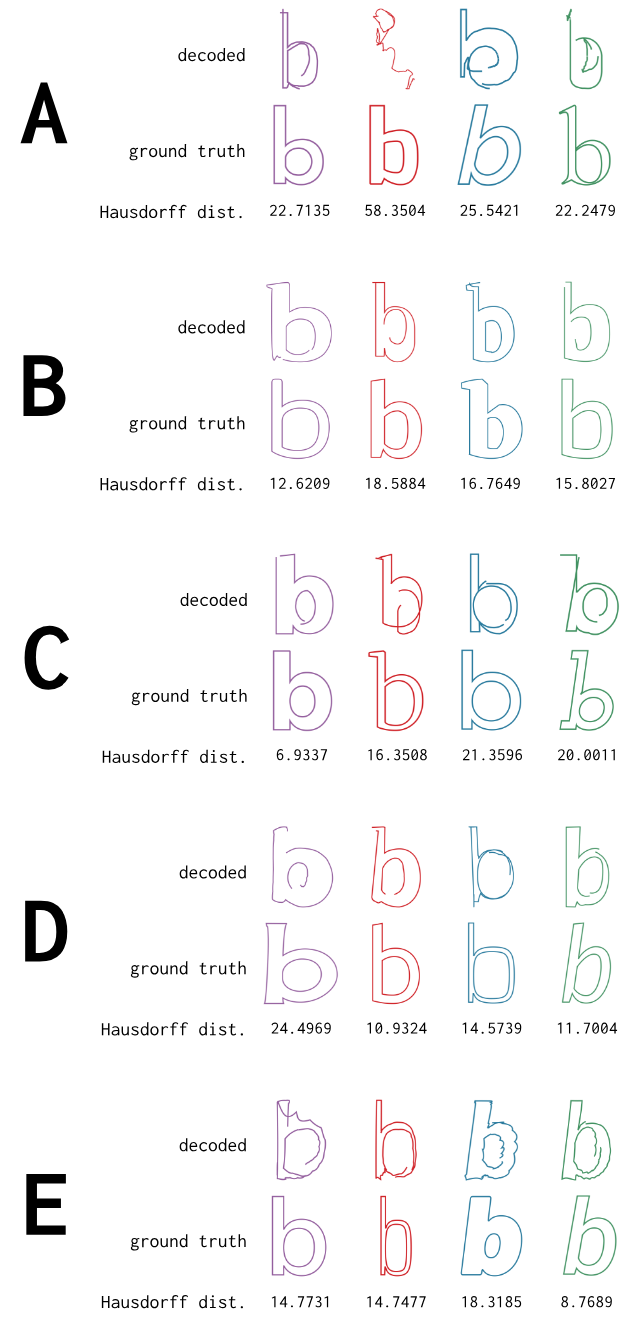
\includegraphics[height=0.8\textheight]{figures/encodings}
    \caption[Visual results of training the SVG model with different encodings]
    {Randomly sampled input-output pairs from the SVG models trained on the five encodings described in Table~\ref{tbl:features}.
    \TODO{resample B}
    Decoded outputs were generated at temperature 0.3.
    Decoded outputs are found in the top row for each encoding, while ground truth inputs are in the bottom row.\label{fig:encodings}}
\end{figure}

